\section{Accelerating ROMs of Non-linear Systems}\label{sec:hyperreduction}

So far, we have pointedly ignored the fact that the Galerkin (Eq.~\ref{eq:galerkinROMODE}), LSPG (Eq.~\ref{eq:lspgLSLin}), and MP-LSVT (Eq.~\ref{eq:mplsvtLSLin}) ROMs \textit{will not generate computational cost savings} for large-scale non-linear systems. This is largely due to the fact that evaluating the non-linear terms $\rhsFunc{\cdot}$ arising from fluxes, source terms, body forces, and boundary conditions still scales with the full-order dimension $\numDOF$. Linear time-invariant systems do not suffer from this issue; given a system of the form $\text{d}\consVec/\text{d}\timeVar - \dummyMat \consVec = \zeroVec$, $\dummyMat \inRTwo{\numDOF}{\numDOF}$, the resulting Galerkin ROM (assuming $\consScale = \resScale = \identMat$) takes the form
%
\begin{equation}
    \ode{\consVecCoef}{\timeVar} = \consTrial^\top \dummyMat \consTrial \consVecCoef.
\end{equation}
%
The matrix $\consTrial^\top \dummyMat \consTrial \consVecCoef \inRTwo{\numConsModes}{\numConsModes}$ can be precomputed in the \textit{offline} stage before evaluating the ROM in the \textit{online} stage. Such a precomputation is impossible for general non-linear systems. The low-dimensional state must first be \textit{lifted} to the full-dimensional state (via $\decoderFunc{\consVecCoef}$) to evaluate the non-linear terms $\rhsFunc{\cdot}$. In the case of Galerkin projection, this term must then be projected onto the tangent trial space before integrating the low-dimensional ODE in time. In the case of LSPG and MP-LSVT ROMs solved via the normal equations, the time-variant test basis must be computed from the residual Jacobian. Despite the fact that the resulting low-dimensional system may be less expensive to temporally integrate, these additional operations often outweigh any cost savings. Particularly for complex multi-physics systems, the evaluation of $\rhsFunc{\cdot}$ accounts for the vast majority of the solver cost, and failing to reduce this cost often fails to reduce the ROM cost below that of the FOM.

To achieve the intended goal of significantly reducing the cost of evaluating the model, we must eliminate the ROM's dependence on the full-order dimension $\numDOF$. Techniques which seek this goal are generally referred to as \textit{hyper-reduction} methods. Most prevalent and mature are so-called \textit{sparse sampling} methods, which evaluate the governing equations or non-linear terms at a small number of carefully selected degrees of freedom. For this reason, throughout the remainder of this thesis we will refer to non-hyper-reduced ROMs as \textit{unsampled ROMs}.

Work in this thesis focuses exclusively on linear sparse-sampling methods for linear subspace ROMs, including missing point estimation~\cite{Astrid2004}, collocation~\cite{Bos2004}, and methods of the \textit{approximate-then-project} type, namely the discrete empirical interpolation method~\cite{Chaturantabut2010} and gappy proper orthogonal decomposition~\cite{Everson1995}. Work on \textit{project-then-approximate} approaches, such as cubature methods~\cite{An2008,Hernandez2017} and the energy-conserving sampling and weighting method~\cite{Farhat2014}, show promise in enhancing the accuracy of hyper-reduced ROMs. To date, however, these methods have been analyzed almost exclusively for finite-element structural dynamics models. Their application to projection-based ROMs of hyperbolic fluid flow systems is still in its early stages~\cite{Grimberg2020Hyper}, and is not analyzed here. Neural network approaches to hyper-reduction~\cite{nnHyperRed} and hyper-reduction for non-linear manifold ROMs~\cite{Kim2022} have been proposed, but are also not analyzed here.

Before proceeding, we define a \textit{sampling operator} $\sampMat \defEq [\canonVec_{\dummyIdx_1}, \; \canonVec_{\dummyIdx_2}, \; \hdots, \; \canonVec_{\dummyIdx_{\numSamps}} ]^\top \inRTwo{\numSamps}{\numDOF}$, which is composed of $\numSamps$ unique canonical unit vectors $\canonVec_{\dummyIdx} \inROne{\numDOF}$. For example, given $\numDOF = 5$, $\numSamps = 3$, $\sampMat = [\canonVec_1, \; \canonVec_3, \; \canonVec_4]$,
and a vector $\dummyVec = [\dummyVecVar_1, \; \hdots, \; \dummyVecVar_5]^\top$, the sampling operation $\sampMat \dummyVec$ is computed as
%
\begin{equation}
	\sampMat \dummyVec =
	\begin{bmatrix}
		1 & 0 & 0 & 0 & 0 \\
		0 & 0 & 1 & 0 & 0 \\
		0 & 0 & 0 & 1 & 0 \\
	\end{bmatrix}
	\begin{bmatrix}
		\dummyVecVar_1 \\ \dummyVecVar_2 \\ \dummyVecVar_3 \\ \dummyVecVar_4 \\ \dummyVecVar_5
	\end{bmatrix} =
	\begin{bmatrix}
		\dummyVecVar_1 \\ \dummyVecVar_3 \\ \dummyVecVar_4
	\end{bmatrix}
\end{equation}
%
Such sampling operations are central to each sparse-sampling method described here, and how the sampling indices are selected may have a drastic effect on the accuracy and robustness of the hyper-reduced ROM. Several algorithms for selecting sampling indices are described later in Section~\ref{subsec:sampleSelect}. We now begin by discussing missing point estimation for Galerkin ROMs and collocation for LSPG and MP-LSVT ROMs, followed by gappy POD for each PROM method.

\subsection{Missing Point Estimation for Galerkin ROMs}

Hyper-reduction via missing point estimation (MPE) was introduced by Astrid and coworkers, first for ROMs of a linear time-varying 2D heat conduction problem~\cite{Astrid2004} and later for a non-linear model of a glass melt feeder~\cite{Astrid2008}. It aims to reduce the computational expense of non-linear ROMs by sampling the governing semi-discrete ODE, followed by Galerkin projection of the ODE via the sampled trial basis. The first step can be written by applying the sampling operator to the full-order ROM ODE (Eq.~\ref{eq:romFullODEMod})
%
\begin{equation}
    \resScaleInv \sampMat \left[\jacobDecode \ode{\consVecCoef}{\timeVar} - \sampMat \rhsFunc{\consVecRom, \; \timeVar}\right] = \zeroVec
\end{equation}
%
Projection by $\sampMat \jacobDecode$ and rearranging terms leads to the equation
%
\begin{equation}
	\ode{\consVecCoef}{\timeVar} = \left[ \left[\sampMat \jacobDecode\right]^\top \resScaleInv \sampMat \jacobDecode\right]^{-1} \left[\sampMat \jacobDecode\right]^\top \resScaleInv \sampMat \rhsFunc{\consVecRom, \; \timeVar}
\end{equation}
%
In this work, we only perform hyper-reduction for linear trial spaces, so substituting $\jacobDecode = \consScale \consTrial$ leads to the form
%
\begin{equation}\label{eq:mpeGalerkinLinear}
	\ode{\consVecCoef}{\timeVar} = \left[ \left[\sampMat \consScale \consTrial \right]^\top \resScaleInv \sampMat \consScale \consTrial \right]^{-1} \left[\sampMat \consScale \consTrial \right]^\top \resScaleInv \sampMat \rhsFunc{\consVecRom, \; \timeVar}
\end{equation}
%
In the case $\consScale = \resScale = \identMat$, this simplifies further to
%
\begin{equation}
	\ode{\consVecCoef}{\timeVar} = \left[ \left[\sampMat \consTrial \right]^\top \sampMat \consTrial \right]^{-1} \left[\sampMat \consTrial \right]^\top \sampMat \rhsFunc{\consVecRom, \; \timeVar}
\end{equation}
%
Note that the matrix inverse term is not equal to the identity matrix, as it did in the unsampled Galerkin ROM in Eq.~\ref{eq:galerkinROMODELinearSimple}, as the matrix $\sampMat \consTrial$ has no guarantee of orthonormality. However, the matrix $\left[ \left[\sampMat \consTrial \right]^\top \sampMat \consTrial \right]^{-1} \left[\sampMat \consTrial \right]^\top \inRTwo{\numConsModes}{\numSamps}$ (or the scaled equivalent for Eq.~\ref{eq:mpeGalerkinLinear}) may be precomputed in the offline stage.

The operation $\sampMat \rhsFunc{\consVecRom, \; \timeVar}$ is the key to cost reduction via the MPE method, whereby only $\numSamps$ elements of the non-linear function $\rhsFunc{\cdot}$ must be evaluated. Similar operations underpin all sparse sampling hyper-reduction methods for PROMs of non-linear systems. In the case $\numSamps \ll \numDOF$, the cost of evaluating the non-linear terms may be drastically reduced. Further, only those mesh elements which are required to compute $\sampMat \rhsFunc{\consVecRom, \; \timeVar}$ must be allocated, potentially greatly reducing the memory consumption of the hyper-reduced ROM relative to the FOM or unsampled ROM. This \textit{sample mesh} concept will be discussed at greater length in Section~\ref{subsec:sampleMesh}.

We mention that a similar method was proposed by Bos \textit{et al.}~\cite{Bos2004} in the context of systems governed by an explicit state space update $\consVec^{\timeIdx} = \rhsFunc{\consVec^{\timeIdx - 1}}$. Their method was proposed at the same time as Astrid~\cite{Astrid2004} and deserves similar credit as it was formulated for general non-linear systems. However, their derivation lacks generality to arbitrary PDEs, and is only equivalent to that of MPE in the specific case of the solution of Eq~\ref{eq:mpeGalerkinLinear} via an explicit time integrator.

\subsection{Collocation for LSPG and MP-LSVT ROMs}

Hyper-reduction of the residual-based PROMs (LSPG and MP-LSVT) by collocation derives from the work by LeGresley~\cite{LeGresley2005}, which applies a similar method to that proposed by MPE for the cost reduction of general non-linear least-squares problems. Given the fully-discrete residual $\resVec$, the least-squares collocation problem is stated as
%
\begin{equation}\label{eq:collocLSPG}
	\consVecCoef^{\timeIdx} = \argmin{\dummyVec \inROne{\numConsModes}} \left\Vert \sampMat \resScaleInv \resFunc{\dummyVec} \right\Vert_2.
\end{equation}
%
By this process, the least-squares minimization problem must only be computed based on the $\numSamps$ sampled elements of the residual. The original work by LeGresley used this procedure exclusively for the solution of steady systems with the goal of accelerating multi-disciplinary optimization problems. The work by Carlberg \textit{et al.}~\cite{Carlberg2013} extended this process to LSPG ROMs, although it was presented as an inferior approach compared to the Gauss--Newton with approximated tensors (GNAT) approach proposed in the paper. The GNAT method is detailed in Section~\ref{subsec:gappyPOD}. We address collocation hyper-reduction for LSPG and MP-LSVT ROMs here.

The solution of Eq.~\ref{eq:collocLSPG} by Gauss--Newton is given as
%
\begin{equation}\label{eq:collocLSPGGauss}
    \delta \consVecCoef^{\newtonIdx} = \argmin{\dummyVec \inROne{\numConsModes}} \left\Vert \sampMat \resScaleInv \left[\jacobRes^{\newtonIdx} \dummyVec - \resFunc{\consVecCoef^{\newtonIdx}}\right] \right\Vert_2,
\end{equation}
\begin{equation}
    \consVecCoef^{\newtonIdx + 1} = \consVecCoef^{\newtonIdx} + \alpha \left[ \delta \consVecCoef^{\newtonIdx} \right].
\end{equation}
%
The normal equations for Eq.~\ref{eq:collocLSPGGauss} is thus given by
%
\begin{equation}
    \left[\testBasisCons^{\newtonIdx}\right]^\top \testBasisCons^{\newtonIdx} \delta \consVecCoef^{\newtonIdx} = -\left[\testBasisCons^{\newtonIdx}\right]^\top \sampMat \resScaleInv \resFunc{\consVecCoef^{\newtonIdx}},
\end{equation}
%
where the test basis is defined as
%
\begin{equation}
    \testBasisCons^\newtonIdx \defEq \sampMat \resScaleInv \jacobCons^\newtonIdx \jacobDecode^{\newtonIdx}.
\end{equation}
%
In the case of a linear trial space, the test basis simplifies to
%
\begin{equation}
    \testBasisCons^\newtonIdx \defEq \sampMat \resScaleInv \jacobCons^\newtonIdx \consScale \consTrial.
\end{equation}
%
In this formulation, we see that only $\numSamps$ elements of the non-linear residual term must by calculated for $\sampMat \resScaleInv \resFunc{\cdot}$. Further, only $\numSamps$ rows of the the residual Jacobian must be calculated for $\sampMat \resScaleInv \jacobCons^\newtonIdx$. As with MPE, this subsampling operation has the capability to drastically reduce the cost of evaluating the LSPG ROM, as the calculation of the non-linear residual and its Jacobian usually dominates the computational cost for solvers of even moderate complexity.

The process for computing the collocated MP-LSVT ROM is, as implied by the unsampled ROM derivation in Section~\ref{sec:mplsvt}, extremely similar to that of collocated LSPG. The non-linear least-squares problem is simply reframed to minimize the residual with respect to the target space modal coefficients, i.e.
%
\begin{equation}\label{eq:collocMPLSVT}
	\primVecCoef^{\timeIdx} = \argmin{\dummyVec \inROne{\numPrimModes}} \left\Vert \sampMat \resScaleInv \resFunc{\dummyVec} \right\Vert_2.
\end{equation}
%
Sparing the reader repetitive derivation details, for a linear trial space the normal equations of the Gauss--Newton solution of Eq.~\ref{eq:collocMPLSVT} is given by
%
\begin{equation}
    \left[\testBasisPrim^{\newtonIdx}\right]^\top \testBasisPrim^{\newtonIdx} \delta \primVecCoef^{\newtonIdx} = -\left[\testBasisPrim^{\newtonIdx}\right]^\top \sampMat \resScaleInv \resFunc{\primVecCoef^{\newtonIdx}},
\end{equation}
%
where the test basis is defined as
%
\begin{equation}
    \testBasisPrim^\newtonIdx \defEq \sampMat \resScaleInv \jacobPrim^\newtonIdx \primScale \primTrial.
\end{equation}
%
Again, we see that only $\numSamps$ rows of the non-linear residual $\sampMat \resScaleInv \resFunc{\cdot}$ and residual Jacobian $\sampMat \resScaleInv \jacobPrim$ must be computed to solve the collocated MP-LSVT ROM.

\subsection{DEIM and GNAT}\label{subsec:gappyPOD}
%
Both hyper-reduction methods presented so far, MPE and collocation, have enabled cost reduction of PROMs simply by sampling the original governing ROM equations and computing the solution normally. However, as shown by Carlberg \text{et al.}~\cite{Carlberg2013}, these methods often generate inaccurate or unstable solutions for convection-dominated fluid flow systems. Alternatively, several methods have been proposed which compute data-driven, approximate reconstructions of non-linear terms based on a small number of samples of the functions. As such, these approaches attempt to incorporate the action of the full-field function, instead of discarding unsampled elements entirely as in MPE or collocation. Because of this, they are sometimes referred to as \textit{function reconstruction} methods.

Two well-established function reconstruction methods are the discrete empirical interpolation method (DEIM) and gappy proper orthogonal decomposition (gappy POD). The two are closely related, but were originally developed for different applications. DEIM, introduced by Chaturantabut and Sorensen~\cite{Chaturantabut2010}, is a discrete formulation of the empirical interpolation method (EIM)~\cite{Barrault2004}. It introduces an approximation of non-linear functions of the form,
%
\begin{equation}\label{eq:deimRHSApprox}
    \resFunc{\dummyVec} \approx \resApproxFunc{\dummyVec} \defEq \deimBasis \left[ \sampMat \deimBasis \right]^{-1} \sampMat \resFunc{\dummyVec},
\end{equation}
%
where we use the residual function $\resVec$ for the sake of notational simplicity, but note that this method extends to approximation of any non-linear function. The matrix $\deimBasis \defEq [\deimBasisVec_1, \; \deimBasisVec_2, \; \hdots, \; \deimBasisVec_{\numResModes}] \inRTwo{\numDOF}{\numResModes}$ is an orthonormal basis, usually generated by POD from FOM snapshots of the non-linear function $\resVec$. It is assumed that the matrix $\sampMat \deimBasis \inRTwo{\numSamps}{\numResModes}$ has full rank. Again, in computing $\resApproxVec$, we see that the non-linear function $\resVec$ must only be sampled at $\numSamps$ degrees of freedom, instead of its full dimension $\numDOF$.

Note that here, the number of DEIM basis modes is equal to the number of sampled degrees of freedom, i.e., $\numSamps = \numResModes$. By this formulation, the non-linear function is interpolated exactly at $\numSamps < \numDOF$ degrees of freedom and interpolated approximately at all other degrees of freedom. The error in this approximation is bounded~\cite{Chaturantabut2010} by the inequality
%
\begin{equation}\label{eq:deimErrorBound}
   \left\Vert \resFunc{\dummyVec} - \resApproxFunc{\dummyVec} \right\Vert_2 \le \left\Vert \left[ \sampMat \deimBasis \right]^{-1} \right\Vert_2 \left\Vert \left[ \identMat - \deimBasis \deimBasis^\top \right] \resFunc{\dummyVec} \right\Vert_2,
\end{equation}
%
where the first norm term on the right-hand side is a measure of the \textit{sampling error}, and the second norm term is the \textit{projection error}. As will be discussed shortly, various methods of selecting the sampling degrees of freedom often attempt to minimize these sources of error.

Again, DEIM is restricted to the case where $\numSamps = \numResModes$. For practical engineering systems, $\numResModes \ll \numDOF$ generally, and such extreme sparse sampling may result in high interpolation error at the unsampled degrees of freedom. Furthermore, Peherstorfer et al.~\cite{Peherstorfer2020} show that increasing $\numResModes$ can lead to an unstable increase in the interpolation error if $\numSamps = \numResModes$. Gappy POD was originally developed well before the advent of DEIM to approximate full field data from a few sparse samples~\cite{Everson1995}, and has seen extensive use in sparse sensor placement~\cite{willcoxGappyPOD,ManoharSparseSensor} and extensions of missing point estimation~\cite{Zimmermann2016}. As such, gappy POD has also been used to approximate non-linear functions in dynamical systems. The method takes a very similar approach to DEIM, but relaxes the restriction on the number of sampled degrees of freedom, allowing $\numSamps \ge \numResModes$. The approximation becomes a least-squares regression of the form
%
\begin{equation}\label{eq:gappyPODRHSApprox}
    \resFunc{\dummyVec} \approx \resApproxFunc{\dummyVec} \defEq \deimBasis \left[ \sampMat \deimBasis \right]^{+} \sampMat \resFunc{\dummyVec},
\end{equation}
%
where the operation $\dummyMat^+$ indicates the Moore--Penrose inverse (or pseudo-inverse). Again, this assumes $\sampMat \deimBasis$, which is now a rectangular matrix, has full column rank. Similarly to Eq.~\ref{eq:deimErrorBound}, the gappy POD regression error is bounded by
%
\begin{equation}\label{eq:gappyPODErrorBound}
    \left\Vert \resFunc{\dummyVec} - \resApproxFunc{\dummyVec} \right\Vert_2 \le \left\Vert \left[ \sampMat \deimBasis \right]^{+} \right\Vert_2 \left\Vert \left[ \identMat - \deimBasis \deimBasis^\top \right] \resFunc{\dummyVec} \right\Vert_2.
\end{equation}
%
For the remainder of this thesis, we will restrict discussion of hyper-reduction to gappy POD, as it is more general than DEIM. We simply remind the reader that in the specific case of $\numResModes = \numConsModes$, gappy POD is equivalent to DEIM.

The approximation of non-linear functions by Eq.~\ref{eq:gappyPODRHSApprox} can be applied to projection-based ROM formulations to vastly reduce the computational cost of evaluating non-linear terms arising from the discretization of the governing equations. Hyper-reduction of Galerkin ROMs by gappy POD is described first, followed by hyper-reduction of LSPG and MP-LSVT ROMs.

\paragraph*{Gappy POD for Galerkin ROMs}\mbox{}\\
%
For Galerkin projection ROMs, the traditional method of gappy POD approximates the non-linear terms $\rhsVec$ as
%
\begin{equation}
	\rhsApproxFunc{\consVec, \; \timeVar} \defEq \deimBasis \left[ \sampMat \deimBasis \right]^+ \sampMat \rhsFunc{\consVec, \; \timeVar}.
\end{equation}
%
Substituting this approximation into the linear subspace Galerkin ROM ODE (Eq.~\ref{eq:galerkinROMODELinear}) results in the hyper-reduced ROM
%
\begin{equation}\label{eq:galerkinROMHR}
    \ode{\consVecCoef}{\timeVar} = \left[\consTrial^\top \consScale \resScaleInv \consScale \consTrial\right]^{-1} \consTrial^\top \consScale \resScaleInv \deimBasis \left[ \sampMat \deimBasis \right]^+ \sampMat \rhsFunc{\consVecRom, \; \timeVar}.
\end{equation}
%
The low-dimensional matrix $\left[\consTrial^\top \consScale \resScaleInv \consScale \consTrial\right]^{-1} \consTrial^\top \consScale \resScaleInv \deimBasis \left[ \sampMat \deimBasis \right]^+ \inRTwo{\numConsModes}{\numSamps}$ can be pre-computed in the offline stage and loaded from disk prior to evaluating the unsteady ROM. Further simplifying, if $\consScale = \resScale = \identMat$, the formulation is greatly reduced to
%
\begin{equation}
    \ode{\consVecCoef}{\timeVar} = \consTrial^\top \deimBasis \left[ \sampMat \deimBasis \right]^+ \sampMat \rhsFunc{\consVecRom, \; \timeVar},
\end{equation}
%
where again, the low-dimensional matrix $\consTrial^\top \deimBasis \left[ \sampMat \deimBasis \right]^+ \inRTwo{\numConsModes}{\numSamps}$ can be precomputed. Gappy POD Galerkin projection ROMs of this form have been successfully applied to a host of non-linear fluid flow problems~\cite{Chaturantabut2011,Stefanescu2013,Wirtz2014,Amsallem2015,Alla2017}.

An alternative method of computing the gappy POD Galerkin ROM is posed by Peherstorfer~\cite{Peherstorfer2020Adaptive}, who reframes the fully discrete O$\Delta$E in the form
%
\begin{equation}\label{eq:benResidual}
	\consVec^{\timeIdx-1} - \rhsResFunc{\consVec^{\timeIdx}, \timeVar} = \zeroVec
\end{equation}
%
where all terms of the time integrator, except for $\consVec^{\timeIdx - 1}$, have been grouped with the non-linear terms $\rhsFunc{\cdot}$ into the lumped $\rhsResFunc{\cdot}$. Note that this is more general than the explicit update discussed by Bos \textit{et al.}~\cite{Bos2004}, as it extends to implicit time integrators as well. This form is, at first glance, confusing, as we normally seek the solution solution at the next time step, $\consVec^{\timeIdx}$, as a function of past time steps, not the other way around as in Eq.~\ref{eq:benResidual}. However, this simply reflects the nature of implicit time integrators, in which the non-linear terms $\rhsVec$ are evaluated at future time steps. For example, the backward Euler (BDF1) time integrator would compute $\rhsResVec$ as
%
\begin{equation}
	\rhsResFunc{\consVec^{\timeIdx}} \defEq \consVec^{\timeIdx} - \dt \rhsFunc{\consVec^{\timeIdx}} \quad \text{(BDF1)}
\end{equation}
%
The approximate non-linear term is then approximated as
%
\begin{equation}
	\rhsResFunc{\consVec} \approx \rhsResApproxFunc{\consVec} \defEq \deimBasis \left[\sampMat \deimBasis \right]^+ \sampMat \rhsResFunc{\consVec}.
\end{equation}
%
Substitution into Eq.~\ref{eq:benResidual} and projection by the tangent trial space leads to an alternative hyper-reduced Galerkin ROM of the form
%
\begin{equation}
    \consVecCoef^{\timeIdx-1} - \left[\jacobDecode^\top \resScaleInv \jacobDecode\right]^{-1} \jacobDecode^\top \resScaleInv \rhsResApproxFunc{\consVecRom^{\timeIdx}} = \zeroVec.
\end{equation}
%
As mentioned previously, the above formulation is fairly non-standard and can be quite confusing for ROM practitioners. However, as will be discussed in Sections~\ref{subsec:regBasis}, this formulation lends itself to a simplification in which the regression basis $\deimBasis$ can be equated to the solution trial basis $\consTrial$ or $\primTrial$. Its use in adaptive bases and sampling is also outlined in Section~\ref{sec:adaptation}.

\paragraph*{GNAT for LSPG and MP-LSVT ROMs}\mbox{}\\
%
Applying gappy POD to LSPG and MP-LSVT ROMs takes an approach akin to that of collocation. Instead of constructing a least-squares regression for the sampled non-linear function $\rhsVec$, however, the complete fully-discrete residual $\resVec$ is approximated and substituted into the residual minimization problem given by Eq.~\ref{eq:lspgLS} or~\ref{eq:mplsvtLS}. We first examine the procedure for LSPG, which was first formulated by Carlberg and coworkers~\cite{Carlberg2010,Carlberg2013}, who referred to the procedure as Gauss--Newton with approximated tensors (GNAT). Substituting the residual approximation into Eq.~\ref{eq:lspgLS} results in the non-linear least-squares problem
%
\begin{equation}\label{eq:lspgLSHR}
    \consVecCoef^{\timeIdx} = \argmin{\dummyVec \inROne{\numConsModes}} \left\Vert \deimBasis \left[ \sampMat \deimBasis \right]^{+} \sampMat \resScaleInv \resFunc{\dummyVec} \right\Vert_2.
\end{equation}
%
Solving Eq.~\ref{eq:lspgLSHR} by Gauss--Newton results in the iterative process
%
\begin{equation}\label{eq:lsgpLinHR}
    \delta \consVecCoef^{\newtonIdx} = \argmin{\dummyVec \inROne{\numConsModes}} \left\Vert \deimBasis \left[ \sampMat \deimBasis \right]^{+} \sampMat \resScaleInv \left[ \jacobRes^{\newtonIdx} \dummyVec - \resFunc{\consVecCoef^{\newtonIdx}}\right] \right\Vert_2,
\end{equation}
\begin{equation}
    \consVecCoef^{\newtonIdx + 1} = \consVecCoef^{\newtonIdx} + \alpha \left[ \delta \consVecCoef^{\newtonIdx} \right].
\end{equation}
%
Solution of Eq.~\ref{eq:lsgpLinHR} via the normal equations is again given by a Petrov--Galerkin ROM of the form
%
\begin{equation}\label{eq:lspgHRSolve}
    \left[ \testBasisCons^\newtonIdx \right]^\top \testBasisCons^\newtonIdx \delta \consVecCoef^{\newtonIdx} = -\left[\testBasisCons^\newtonIdx \right]^\top \deimBasis \left[ \sampMat \deimBasis \right]^{+} \sampMat \resScaleInv \resFunc{\consVecCoef^{\newtonIdx}}.
\end{equation}
%
where the test basis is defined as
%
\begin{equation}\label{eq:lspgHRTest}
    \testBasisCons^\newtonIdx \defEq \deimBasis \left[ \sampMat \deimBasis \right]^{+} \sampMat \resScaleInv \jacobCons^{\newtonIdx} \jacobDecode^{\newtonIdx}.
\end{equation}
%
The original work on GNAT~\cite{Carlberg2013} suggests an alternative formulation, whereby separate regression bases are computed for the residual and residual Jacobian, denoted by $\deimBasisRes \inRTwo{\numDOF}{\numResModes}$ and $\deimBasisJacob \inRTwo{\numDOF}{\numJacobModes}$ respectively. Equation~\ref{eq:lsgpLinHR} can thus be written as
%
\begin{equation}\label{eq:separateBasesGNAT}
    \delta \consVecCoef^{\newtonIdx} = \argmin{\dummyVec \inROne{\numConsModes}} \left\Vert \deimBasisJacob \left[ \sampMat \deimBasisJacob \right]^{+} \sampMat \resScaleInv \jacobRes^{\newtonIdx} \dummyVec - \deimBasisRes \left[ \sampMat \deimBasisRes \right]^{+} \sampMat \resScaleInv \resFunc{\consVecCoef^{\newtonIdx}} \right\Vert_2,
\end{equation}
%
In practice, choosing $\deimBasisRes \neq \deimBasisJacob$ has not been observed to generate hyper-reduced ROMs which are drastically better than those generated by choosing $\deimBasisRes = \deimBasisJacob$. The added computational complexity makes it difficult to justify implementing Eq.~\ref{eq:separateBasesGNAT}. As such, for all results presented in this thesis we choose $\deimBasisRes = \deimBasisJacob$.

Hyper-reduction of MP-LSVT ROMs via gappy POD follow an extremely similar method, beginning from the fully-discrete residual minimization with respect to the target state latent variables,
%
\begin{equation}
    \primVecCoef^{\timeIdx} = \argmin{\dummyVec \inROne{\numPrimModes}} \left\Vert \deimBasis \left[ \sampMat \deimBasis \right]^{+} \sampMat \resScaleInv \resFunc{\dummyVec} \right\Vert_2.
\end{equation}
%
Solution via Gauss--Newton and the normal equations results in a similar hyper-reduced Petrov--Galerkin formulation of
%
\begin{equation}\label{eq:mplsvtHRSolve}
    \left[ \testBasisPrim^\newtonIdx \right]^\top \testBasisPrim^\newtonIdx \delta \primVecCoef^{\newtonIdx} = -\left[\testBasisPrim^\newtonIdx \right]^\top \deimBasis \left[ \sampMat \deimBasis \right]^{+} \sampMat \resScaleInv \resFunc{\primVecCoef^{\newtonIdx}},
\end{equation}
%
with the test basis
%
\begin{equation}\label{eq:mplsvtHRTest}
    \testBasisPrim^\newtonIdx \defEq \deimBasis \left[ \sampMat \deimBasis \right]^{+} \sampMat \resScaleInv \jacobPrim^{\newtonIdx} \jacobDecode^{\newtonIdx}.
\end{equation}
%
Only $[ \sampMat \deimBasis ]^{+} \inRTwo{\numResModes}{\numSamps}$ is pre-computed offline. Although the matrix $\deimBasis [ \sampMat \deimBasis ]^{+} \inRTwo{\numDOF}{\numSamps}$ can be pre-computed offline, a matrix of $\numDOF \times \numSamps$ elements can be prohibitively large for high-dimensional systems and may not be possible to store in memory. Further, substitution of Eq.~\ref{eq:mplsvtHRTest} into Eq.~\ref{eq:mplsvtHRSolve} and recognizing the product $\deimBasis^\top \deimBasis = \identMat$ eliminates the need to precompute $\deimBasis [ \sampMat \deimBasis ]^{+}$.

As with collocation, we see that computing the sampled residual $\sampMat \resFunc{\cdot}$ only requires that the residual be evaluated at $\numSamps$ degrees of freedom. Further, in Eqs.~\ref{eq:lspgHRTest} and~\ref{eq:mplsvtHRTest} we see that only the corresponding $\numSamps$ rows of the residual Jacobians $\jacobCons $ and $\jacobPrim$ need to be computed. Thus, the hyper-reduced ROM is truly independent of the FOM dimension $\numDOF$. When $\numSamps \ll \numDOF$ and evaluation of the non-linear terms accounts for a majority of the computational burden, this sparse sampling has the potential to drastically reduce the cost of the hyper-reduced ROM relative to the FOM. Our work has recorded four orders of magnitude cost reduction for a three-dimensional model rocket combustor~\cite{Wentland2021}. Up to five orders of magnitude cost reduction has been recorded~\cite{Grimberg2021}, consuming a few core-hours to compute a ROM where the equivalent FOM simulation consumed over two thousand core-weeks. Such cost savings bring projection-based ROMs into the realm of possibility for many-query applications.

\subsection{Regression Basis Calculation}\label{subsec:regBasis}
%
We now address the question of how the regression basis $\deimBasis$ is computed. Although the process generally mirrors that of computing the solution trial bases $\consTrial$ or $\primTrial$, there are several approaches for computing $\deimBasis$ which are suggested by the literature and deserve explanation.

\paragraph*{Galerkin RHS Approximation}\mbox{}\\
%
In the case of gappy POD Galerkin ROMs, we have already explicitly outlined the two approximations of non-linear terms in the ROM ODE/O$\Delta$E, which we restate here. The traditional method of gappy POD for Galerkin projection ROMs~\cite{Chaturantabut2010} computes a regression for the non-linear function $\rhsFunc{\cdot}$ of the form
%
\begin{equation}
	\rhsFunc{\consVec, \timeVar} \approx \rhsApproxFunc{\consVec, \timeVar} \defEq \deimBasis \left[\sampMat \deimBasis \right]^+ \sampMat \rhsFunc{\consVec, \timeVar}
\end{equation}
%
In this case, as with computing the solution trial bases, snapshots of the unsteady non-linear term field $\rhsFunc{\consVec, \timeVar}$ are collected from FOM simulations. Unlike the process for the solution trial bases, we do not define a reference state about which snapshots are centered. However, disparate scales of the non-linear terms must be accounted for, and we suggest using the same scaling format as that used for scaling the fully-discrete residual, $\resScaleInv$. The snapshot matrix is thus aggregated as
%
\begin{equation}
	\rhsDataMat = \left[ \resScaleInv \rhsFunc{\consFunc{\timeVar^0}}, \; \resScaleInv \rhsFunc{\consFunc{\timeVar^1}}, \; \hdots, \; \resScaleInv \rhsFunc{\consFunc{\finalTime}} \right]
\end{equation}
%
The regression basis is then computed from the POD of the snapshot matrix $\rhsDataMat$, extracting the leading $\numResModes$ singular vectors as $\deimBasis$.

\paragraph*{State Approximation}\mbox{}\\
%
The method of Peherstorfer~\cite{Peherstorfer2020Adaptive}, as previously discussed in Section~\ref{subsec:gappyPOD}, reframes the fully-discrete residual as
%
\begin{equation}\label{eq:benResidualTwo}
	\consVec^{\timeIdx-1} - \rhsResFunc{\consVec^{\timeIdx},\; \timeVar^{\timeIdx}} = \zeroVec
\end{equation}
%
Although this formulation may seem non-intuitive, it is only a grouping of terms arising from the implicit time integration of the governing ODE. Interestingly, treating the lumped non-linear term $\rhsResFunc{\cdot}$ as the non-linear function to be approximated makes the connection
%
\begin{equation}\label{eq:benResidualApprox}
	\consVec^{\timeIdx-1} \approx \rhsResApproxFunc{\consVec} \defEq \deimBasis \left[\sampMat \deimBasis \right]^+ \sampMat \rhsResFunc{\consVec}
\end{equation}
%
At first glance, this formulation might suggests that we can use the solution trial basis as the regression basis; that is, $\deimBasis = \consTrial$. However, this is not entirely accurate, as the state representation is given as $\consVecRom \defEq \consVecCent + \consScale \consTrial \consVecCoef$. Attempting to directly approximate this vector by gappy POD results in
%
\begin{equation}\label{eq:stateGPODWrong}
	\consVec \approx \consVecCent + \consScale \consTrial \left[\sampMat \consScale \consTrial\right]^+ \sampMat \left[\consVec - \consVecCent\right]
\end{equation}
%
which is not appropriate for use in Eq.~\ref{eq:benResidualApprox}. The governing system in Eq.~\ref{eq:benResidual} requires some manipulation to achieve a more appropriate gappy POD approximation.

We will restrict discussion to linear multi-step methods, which normally take the general form
%
\begin{equation}\label{eq:lms}
	\consVec^{\timeIdx} + \sum_{\dummyIdx=1}^{s} a_{\dummyIdx} \consVec^{\timeIdx-\dummyIdx} + \dt \sum_{\dummyIdx=0}^{s} b_{\dummyIdx} \rhsFunc{\consVec^{\timeIdx-\dummyIdx}, \; \timeVar^{\timeIdx-\dummyIdx}} = \zeroVec
\end{equation}
%
where $b_{\dummyIdx}$, $a_{\dummyIdx} \in \mathbb{R}$ are tabulated coefficients for a given method of order $s$. We note that for a linear multistep method to be consistent, the coefficients $a_{\dummyIdx}$ must satisfy
%
\begin{equation}\label{eq:lmsNegOne}
	\sum_{\dummyIdx=1}^{s} a_{\dummyIdx} = -1
\end{equation}
%
Substituting the linear trial space representation $\consVec \defEq \consVecCent + \consScale \consTrial \consVecCoef$ into Eq.~\ref{eq:lms}, and recognizing that $\consVecCent + \consVecCent \sum_{\dummyIdx=1}^{s} a_{\dummyIdx} = \zeroVec$ by Eq.~\ref{eq:lmsNegOne}, we can rewrite the fully-discrete residual to match the form in Eq.~\ref{eq:benResidualTwo} as
%
\begin{equation}
	\consScale \consTrial \consVecCoef^{\timeIdx-1} + \consScale \consTrial \left[\frac{1}{a_1} \consVecCoef^{\timeIdx} + \sum_{\dummyIdx=2}^{s} \frac{a_{\dummyIdx}}{a_1} \consVecCoef^{\timeIdx-\dummyIdx}\right] + \dt \sum_{\dummyIdx=0}^{s} \frac{b_{\dummyIdx}}{a_1} \rhsFunc{\consVecRom^{\timeIdx-\dummyIdx}, \; \timeVar^{\timeIdx-\dummyIdx}} = \zeroVec
\end{equation}
%
where we can define the lumped non-linear term as
%
\begin{equation}
	-\rhsResFunc{\consVecCoef^{\timeIdx},\; \timeVar^{\timeIdx}} \defEq \consScale \consTrial \left[\frac{1}{a_1} \consVecCoef^{\timeIdx} + \sum_{\dummyIdx=2}^{s} \frac{a_{\dummyIdx}}{a_1} \consVecCoef^{\timeIdx-\dummyIdx}\right] + \dt \sum_{\dummyIdx=0}^{s} \frac{b_{\dummyIdx}}{a_1} \rhsFunc{\consVecRom^{\timeIdx-\dummyIdx}, \; \timeVar^{\timeIdx-\dummyIdx}}
\end{equation}
%
Given the resulting equivalence
%
\begin{equation}
	\consScale \consTrial \consVecCoef^{\timeIdx-1} = \rhsResFunc{\consVecCoef^{\timeIdx},\; \timeVar^{\timeIdx}},
\end{equation}
%
it now appears appropriate to approximate the lumped non-linear term as $\rhsResApproxFunc{\cdot} \defEq \deimBasis \left[\sampMat \deimBasis\right]^+ \sampMat \rhsResFunc{\cdot}$ by choosing $\deimBasis = \consScale \consTrial$. Although this derivation may seem tedious to make this distinction solely in the context of linear multistep time integrators, we recall that the attempt to naively set $\deimBasis = \consTrial$ for any time integration scheme resulted in the unusable gappy POD approximation given in Eq.~\ref{eq:stateGPODWrong}.

The usefulness of this formulation lies solely in
{\color{red} INCOMPLETE, NO JUSTIFICATION FOR MP-LSVT}

\paragraph*{Residual Approximation}\mbox{}\\
%
{\color{red} FINISH}

\subsection{Sample Selection}\label{subsec:sampleSelect}

As described above, the computation of the non-linear function regression basis $\deimBasis$ is somewhat nuanced, but is ultimately derived from the POD of a solution, non-linear terms, or fully-discrete residual snapshot matrix. Methods for selecting sampling indices, and hence the construction of the sampling operator $\sampMat$, are much more varied. The selection of $\numSamps > \numResModes$ samples which globally minimize the regression error (Eq.~\ref{eq:gappyPODErrorBound}) is a computationally-intractable problem. As such, almost all methods for selecting sampling points are \textit{greedy} methods, which iteratively select points based on some measure of local optimality at a given iteration. The ``best'' choice of local error measure, and hence greedy sampling method, is an area of active research. Unfortunately, very few comparisons between sampling methods have been published, with the exception of the work by Peherstorfer \textit{et al.}~\cite{Peherstorfer2020}. Although extremely insightful, their exploration of hyper-reduced ROMs was limited to simple one-dimensional steady reaction-diffusion system. Results presented in Chapter~\ref{chap:CavityAndCVRC} seek to expand on their work by studying more complex, unsteady 2D and 3D multi-scale and multi-physics problems.

\paragraph*{Sampling Criteria}\mbox{}\\
%
Before discussing specific sampling algorithms, we must address how sampling criteria for greedy algorithms are evaluated. In general, at each greedy iteration, the algorithm chooses the next index to include in the sample set by evaluating some metric (usually an error measure) and selecting the index which maximizes/minimizes that metric. This process is slightly nuanced for the sampling of non-linear functions describing flow physics characterized by disparate spatio-temporal scales. Up until this point, we have spoken about sampling only in terms of individual \textit{degrees of freedom} (DOFs). That is, we have considered sampling indices $\dummyIdx \in \{1,\; \hdots, \; \numDOF\}$ which have no specific connection to any variables or mesh elements. In reality, these indices are important for determining local connectivity of mesh elements and for computing numerical quantities such as fluxes and gradients. A state vector (or a function of the state vector) might be visualized as a two-dimensional array, with the leading dimension corresponding to the number of mesh elements $\numCells$ and the trailing dimension corresponding to the number of variables $\numVars$ associated with a single mesh element. This can be written as
%
\begin{equation}\label{eq:stateMat}
	% right arrow, because I don't want to use equality
	\stateVec \rightarrow
	\begin{bmatrix}
		\stateVar_{1,1} & \hdots & \stateVar_{1,\numVars} \\
		\vdots & \ddots & \vdots \\
		\stateVar_{\numCells,1} & \hdots & \stateVar_{\numCells,\numVars}
	\end{bmatrix}
\end{equation}
%
In this work, we construct the corresponding one-dimensional vector by flattening Eq.~\ref{eq:stateMat} along the leading dimension, result in the form
%
\begin{equation}
	\stateVec \defEq \left[\stateVar_{1,1}, \hdots, \stateVar_{\numCells,1},\stateVar_{1,2}, \hdots, \stateVar_{1,\numVars-1}, \stateVar_{1,\numVars}, \hdots, \stateVar_{\numCells,\numVars} \right]^\top
\end{equation}
%
For a given mesh element index $j \in \{1,\; \hdots,\; \numCells\}$, all DOF indices in $\stateVec$ for the associated state variables can be retrieved as the set $\dummyIdx \in \{j + (k-1) \numCells \; \vert \; 1 \le k \le \numVars \}$.

As will be discussed in more detail in Section~\ref{subsec:sampleMesh}, sampling individual degrees of freedom of a non-linear function usually requires that additional, auxiliary degrees of freedom also be sampled in order to correctly compute the approximated non-linear function. The union of the sampling operator and these auxiliary degrees of freedom can thus be defined as $\sampMatFull \inRTwo{\numSampsFull}{\numDOF}$, and the sampled non-linear function is computed as $\sampMat \rhsFunc{\stateVec} = \rhsFunc{\sampMatFull \stateVec}$. This understanding that additional degrees of freedom must be included in the calculation can influence how greedy sampling metrics are calculated. Three distinct approaches are described below.

\begin{enumerate}
	\item \textit{Agnostic}: The agnostic approach is the simplest sampling criterion, whereby the greedy metric is computed for every unsampled DOF, and only one DOF index is added to the sample set at every greedy iteration. That one DOF is then excluded from all future greedy metric evaluations. Only after $\numSamps$ DOFs have been selected for $\sampSet$ are the auxiliary DOFs appended to the full sample set $\sampSetFull$.
	\item \textit{Post-sampling}: The post-sampling method, as with the agnostic approach, computes the greedy sampling metric at every unsampled DOF and selects one index to append to the sample set $\sampSet$. However, post-sampling also appends all DOFs associated with the mesh element corresponding to the sampled DOF. For example, if there are five variables associated with each mesh element, then five DOFs in total will be appended to the sample set at every greedy iteration. All DOFs associated with that mesh element are then excluded from future greedy metric evaluations, and the process continues until $\numSamps$ indices are included in the sample set.
	\item \textit{Comprehensive}: The comprehensive method, as with the previous two methods, evaluates the greedy metric at all unsampled degrees of freedom, but then sums the greedy metric for all DOFs associated with a given mesh element. That is, a single greedy metric is evaluated for each mesh element. The mesh element which maximizes/minimizes the greedy metric is sampled, corresponding to appending all degrees of freedom associated with the mesh element to the sample set $\sampSet$. Again, this is repeated until all $\numSamps$ degrees of freedom are selected.
\end{enumerate}

The post-sampling and comprehensive methods are motivated by the fact that for coupled fluid flow systems, all degrees of freedom associated with a cell must be included in the auxiliary sample set $\sampSetFull$ if even one degree of freedom is sampled by a greedy algorithm. In this sense, they are a sunk cost in evaluating $\sampMat \rhsFunc{\cdot}$, and assessing their contribution to the greedy sampling metric provides a more complete description.

To the best of the author's knowledge, much of the literature does not discuss such nuances in evaluating the sampling criteria, as most of the theoretical work has dealt with single-variable systems which do not require these considerations. Anecdotally, it seems that much contemporary work pursues the agnostic approach. {\color{red}TALK ABOUT LITERATURE}

% The present  work implements a slightly different approach. At each sampling iteration, only greedy selection metrics for individual degrees of freedom are considered. However, once a single degree of freedom is selected and the associated canonical unit vector is appended to $\sampMat$, all other degrees of freedom associated with this same mesh element are also appended to $\sampMat$. These additional degrees of freedom are then excluded from selection in subsequent sampling iterations. Thus, each iteration of a given sampling algorithm selects all degrees of freedom at a single mesh element, but does not consider the contribution of all of those degrees of freedom in the greedy selection metric. In implementing these algorithms, a sampling rate percentage $\alpha \in [0, \; 1]$ of the total mesh elements to sample is specified, and each sampling iteration selects the degrees of freedom associated with a single mesh element until the desired percentage of mesh elements is sampled. As a result, the total number of degrees of freedom sampled is $\numSamps = \alpha \times \times \numVars$. This approach is more similar to that taken by Zhou~\cite{Zhou2012}. We take care to note that this approach is not optimal, and that the mesh element-based approach described by~\cite{Carlberg2013} is logically a more principled approach to the greedy selection methodology. Future work will explore the performance differences between hyper-reduced ROMs using these two approaches.

As an aside, prior work~\cite{Carlberg2013} has noted that it is important to sample at least one mesh element at each inlet and outlet boundary to facilitate the communication of information from outside of the domain to the other sampled cells. Although this consideration is logical, it is not applied in this work. As will be seen later, this omission does not appear to affect the accuracy and robustness of the hyper-reduced ROMs presented. Whether this is more generally true or a pleasant coincidence is unknown.

\paragraph*{Sampling Algorithms}\mbox{}\\
%
{\color{red} ALGORITHMS}
We now turn to specific algorithms for selecting samples for hyper-reduction. In this thesis, we study random sampling, DEIM-like sampling, eigenvector-based sampling, and determinant-based sampling, which are each detailed in turn.

For all sampling algorithms, the first $\numResModes$ sampled degrees of freedom are selected by the \textit{QDEIM} procedure proposed by Drma\v{c} and Gugercin~\cite{Drmac2016}. In the context of DEIM ROMs ($\numResModes = \numSamps$), this has been shown to exhibit tighter error bounds on the resulting interpolant over the traditional DEIM greedy sampling procedure. As such, each algorithm described here must only select $\numSamps - \numResModes$ samples. This is largely done to maintain consistency between algorithms, some of which require an initial set of sampling points and others which do not.

\begin{enumerate}
	\item \textit{Random Sampling}: By far the simplest method, random sampling randomly selects $\numSamps - \numResModes$ degrees of freedom using a random shuffle \CC routine. Peherstorfer \textit{et al.}~\cite{Peherstorfer2020} provide probabilistic analyses to show that randomized oversampling limits the growth in regression error as the regression dimension $\numResModes$ is increased, even in the presence of additional system noise. Although this method has been observed to generate reasonable reconstructions of unsteady flow fields from a few samples, it often leads to poor results for hyper-reduced ROMs of reacting flows~\cite{Wentland2021}. However, the simplicity of this method can be appealing, as it requires no complex computations or distributed-memory software for large datasets. The computational burden of the offline cost is thus strictly limited to the precomputation of $\left[\sampMat \deimBasis\right]^+$, which is universal to all sampling methods presented here.

	\item \textit{DEIM-like Sampling}: The DEIM-like sampling strategy follows the greedy sampling method originally proposed for DEIM~\cite{Chaturantabut2010} and extended to gappy POD by several researchers~\cite{Zhou2012,Carlberg2013}. This method seeks to minimize the error in computing the regression of the basis vectors $\deimBasisVec_{\dummyIdx}$ themselves. Following a greedy approach, at each sampling iteration $\greedyIdx$ the regression error is calculated by
	%
	\begin{equation}
		\errVec_{\greedyIdx} = \deimBasisVec_{\dummyIdx} - \deimBasis_{\dummyIdxTwo} \left[ \sampMat_{\greedyIdx} \deimBasis_{\dummyIdxTwo} \right]^+ \sampMat_{\greedyIdx}\deimBasisVec_{\dummyIdx},
	\end{equation}
	%
	where the index $\dummyIdx$ repeatedly loops through the integer interval $\{1, \hdots, \; \numResModes\}$ (the greedy element of this approach), and $\deimBasis_{\dummyIdxTwo} \inRTwo{\numDOF}{\dummyIdxTwo}$ contains the leading $\dummyIdxTwo$ basis vectors of $\deimBasis$. The index $\dummyIdxTwo$ begins at 1 and is incremented by one at every sampling loop, until $\dummyIdxTwo = \numResModes$. At every iteration, the degree of freedom for which the absolute error $|\errVec_{\greedyIdx}|$ is greatest is sampled, and the corresponding canonical unit vector appended to $\sampMat_{\greedyIdx}$. For DEIM interpolations, Chaturantabut and Sorensen~\cite{Chaturantabut2010} showed that this algorithm limits the growth of the error bounds in Eq.~\ref{eq:deimErrorBound} at every iteration $\greedyIdx$.

	The algorithm for DEIM-like sampling is provided in Alg.~\ref{alg:deimSampling}.

	\item \textit{Eigenvector-based Sampling}: Eigenvector-based sampling seeks to minimize the sampling error term in Eq.~\ref{eq:gappyPODErrorBound} via a greedy approach. This method is a simplification by Peherstorfer et al.~\cite{Peherstorfer2020} of a greedy sampling procedure by Zimmermann and Willcox~\cite{Zimmermann2016} (Algorithm 4), who originally developed the method in the context of missing point estimation. Some of the motivating theory behind the modified algorithm is reproduced here with permission.

	To select the remaining $\numSamps - \numResModes$ points, the method leverages the fact that by nature of the $\ell^2$ norm, the sampling error may be rewritten as
	%
	\begin{equation}
		\left\Vert \left[ \sampMat \deimBasis \right]^+ \right\Vert_2 = \singVal_{\text{max}} \left( \left[\sampMat \deimBasis \right]^+ \right) = \frac{1}{\singVal_{\text{min}} \left( \sampMat \deimBasis \right)},
	\end{equation}
	%
	where $\singVal_{\text{max}}$ and $\singVal_{\text{min}}$ indicate the maximum and minimum singular values of their arguments, respectively. Thus, at the $\greedyIdx$th sampling iteration, the row of $deimBasis$ is selected which maximizes the smallest singular value (equivalently, the smallest eigenvalue) of $\sampMat_{\greedyIdx} \deimBasis \inRTwo{\greedyIdx}{\numResModes}$ via a symmetric rank-one update. Here, $\sampMat_{\greedyIdx} \inRTwo{\numDOF}{\greedyIdx}$ is the selection matrix constructed from the $\greedyIdx$ unit vectors selected up to iteration $\greedyIdx$ by the greedy procedure. It is shown in~\cite{Peherstorfer2020} that the bounds on this update of the smallest eigenvalue, $\eigenVal_{\numResModes}$, from update step $\greedyIdx$ to $\greedyIdx+1$, is given by
	%
	\begin{equation}\label{eq:gappyPODEStrictBounds}
		\eigenVal_{\numResModes}^{\greedyIdx+1} \ge \eigenVal_{\numResModes}^{\greedyIdx} + \frac{1}{2} \left[ g + \left\Vert \deimBasisREvecRow \right\Vert_2^2 - \sqrt{\left[ g + \left\Vert \deimBasisREvecRow \right\Vert_2^2 \right]^2 - 4g\left[ \left[\mathbf{z}_{\numResModes}^{\greedyIdx} \right]^\top \deimBasisREvecRow \right]^2} \right],
	\end{equation}
	%
	where $g = \eigenVal_{\numResModes-1}^{\greedyIdx} - \eigenVal_{\numResModes}^{\greedyIdx}$, and $\mathbf{z}_{\numResModes}^{\greedyIdx} \inROne{\numResModes}$ is the eigenvector associated with eigenvalue $\eigenVal_{\numResModes}^{\greedyIdx}$ (simply the $\numResModes$th canonical unit vector here). Here, $\deimBasisREvecRow = \rightEvecMat_{\greedyIdx}^\top \deimBasisRowUpdate^\top \inROne{\numResModes}$ is defined for simplification, where $\rightEvecMat_{\greedyIdx}$ are the right singular vectors of $\sampMat_{\greedyIdx}^\top \deimBasis$, and $\deimBasisRowUpdate \inRTwo{1}{\numResModes}$ is the row of $\deimBasis$ to be included at greedy iteration $\greedyIdx$. Previous pre-print versions of~\cite{Peherstorfer2020} offer a simplification of the bound in Eq.~\ref{eq:gappyPODEStrictBounds}, given by
	%
	\begin{equation}\label{eq:gappyPODESimpleBounds}
		\eigenVal_{\numResModes}^{\greedyIdx+1} \ge \eigenVal_{\numResModes}^{\greedyIdx} + \frac{g \left[ [\mathbf{z}_{\numResModes}^\greedyIdx]^\top \deimBasisREvecRow \right]^2}{g + \left\Vert \deimBasisREvecRow \right\Vert_2^2}.
	\end{equation}
	%
	Maximizing this bound on $\eigenVal_{\numResModes}^{\greedyIdx+1}$ is thus equivalent to choosing the basis row $\deimBasisRowUpdate$ which maximizes $(\mathbf{z}_{\numResModes}^{\greedyIdx})^\top \deimBasisREvecRow$ at each greedy iteration. In this work, we choose to follow the bounds in Eq.~\ref{eq:gappyPODESimpleBounds}, in contrast to the bounds in Eq.~\ref{eq:gappyPODEStrictBounds}, as the former leads to a simpler algorithm which is more efficient when working with high-dimensional data in a distributed-memory setting.

	The algorithm for eigenvector-based sampling is provided in Alg.~\ref{alg:eigSampling}.

	\item \textit{Determinant-based Sampling}:

	The algorithm for determinant-based sampling is provided in Alg.~\ref{alg:eigSampling}.

\end{enumerate}

\begin{algorithm}
	\caption{DEIM-like sampling}\label{alg:deimSampling}
	\begin{algorithmic}
		\STATE temp
	\end{algorithmic}
\end{algorithm}

\begin{algorithm}
    \caption{Eigenvector-based sampling}\label{alg:eigSampling}
    \begin{algorithmic}
		\STATE temp
    \end{algorithmic}
\end{algorithm}

\begin{algorithm}
    \caption{Determinant-based sampling}\label{alg:detSampling}
    \begin{algorithmic}
		\STATE temp
    \end{algorithmic}
\end{algorithm}

\subsection{The Sample Mesh}\label{subsec:sampleMesh}

As mentioned in Section~\ref{}, sampling individual degrees of freedom of a non-linear function is not equivalent to sampling the state variable arguments associated with those degrees of freedom, e.g., $\sampMat \resFunc{\consVec} \neq \resFunc{\sampMat \consVec}$. Specifically, the evaluation of the non-linear function at a specific degree of freedom often requires access to all state variables at that point in space. For example, solving the continuity equation of the Navier--Stokes equations at a single discrete point in space requires access to both the density and the velocity field. Further, the state at entirely different points in space may also need to be sampled, e.g., to compute fluxes or gradients.

We visualize this in Fig.~\ref{fig:IBlankConfig} in the context of a cell-centered finite volume discretization with quadrilateral/hexahedral control volumes, with a second-order accurate flux scheme. In this image, the blue cell indicates a control volume where at least one degree of freedom of the non-linear function is to be computed. We refer to this type of cell as a \textit{directly sampled} cell. Red cells, or \textit{flux} cells, are those which share a cell face with directly sampled cells and are required for computing fluxes through the shared faces. Yellow cells are those which are required for computing gradients for second-order state reconstructions at cell faces, or for reconstruction of the state at directly sampled cell vertices. These are referred to as \textit{gradient/vertex} cells. We refer to the flux and gradient/vertex cells as \textit{auxiliary} cells, as they are required for calculating the directly sampled degrees of freedom but are not directly sampled themselves. For two-dimensional simulations, each directly sampled cell is accompanied by four flux cells and eight gradient/vertex cells. For three-dimensional simulations, this increases to six flux cells and 26 gradient/vertex cells per directly sampled cell. These numbers are obviously lower for directly sampled cells near physical domain boundaries.

\begin{figure}
    \centering
    \begin{minipage}{0.45\linewidth}
        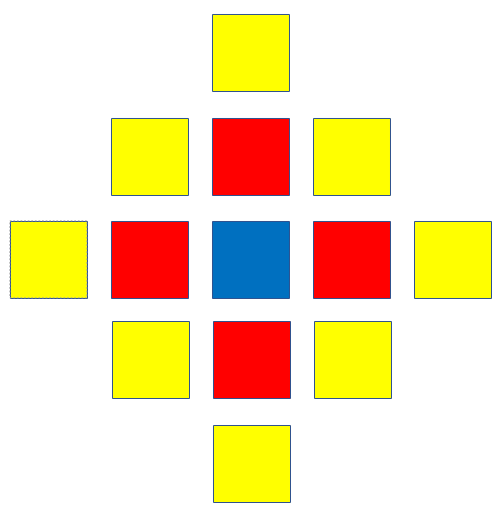
\includegraphics[width=0.99\linewidth]{Chapters/ProjROMs/Images/sampling_2d_2ndOrder.png}
    \end{minipage} \hspace{0.5em}
    \centering
    \begin{minipage}{0.52\linewidth}
        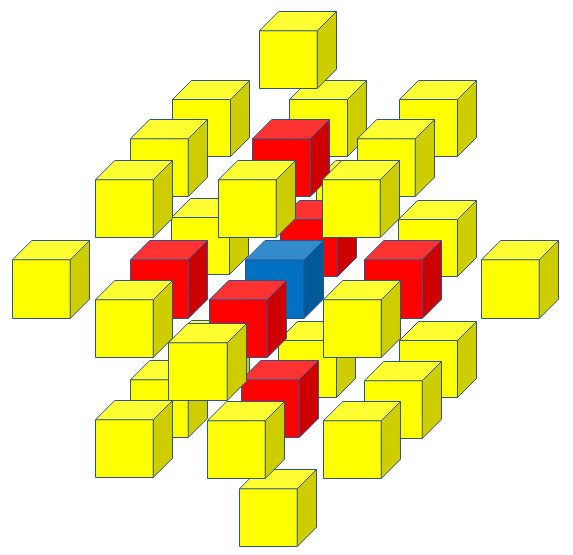
\includegraphics[width=0.99\linewidth]{Chapters/ProjROMs/Images/sampling_3d_2ndOrder.png}
    \end{minipage}
    \caption{\label{fig:IBlankConfig}Sampling schemes for 2nd-order flux scheme in 2D (left) and 3D (right).\\Blue cells are directly sampled, red are flux cells, and yellow are gradient/vertex cells.}
\end{figure}

At each of these cells, the fluid state ($\consVecRom$ and/or $\primVecRom$), trial basis ($\consTrial$ or $\primTrial$) and centering state ($\consVecCent$ or $\primVecCent$), must be held in memory. At directly sampled and flux cells, any thermodynamic/transport properties and state gradients must also be held in memory and calculated at every sub-iteration of the solver. This gives a sense of how rapidly the computational cost and memory consumption can increase with increased sampling. Furthermore, one should not expect a linear correlation between the sampling rate and the resulting computational cost of the hyper-reduced ROM.

Note, however, that for $\numSamps \ll \numDOF$, the solution to the hyper-reduced ROMs (Eqs.~\ref{eq:galerkinROMHR}, \ref{eq:lspgHRSolve}, and~\ref{eq:mplsvtHRSolve}) do not require access to the full $\numDOF$-dimensional state. Indeed, the low-dimensional latent state $\consVecCoef$, $\primVecCoef$ can be advanced in time using only sampled degrees of freedom and those auxiliary degrees of freedom required to evaluate $\sampMat \resFunc{\cdot}$. The full-dimensional state $\consVecRom$, $\primVecRom \inROne{\numDOF}$ can be reconstructed \textit{after} the hyper-reduced ROM has been computed. This motivates the idea of the \textit{sample mesh} concept discussed by Carlberg \textit{et al.}~\cite{Carlberg2013}: only those mesh elements and associated state variables that are strictly required to compute $\sampMat \resFunc{\cdot}$ must be allocated in memory. Those mesh elements, state variables, and additional variables which are not required are simply not allocated. An example of a sample mesh for the transonic cavity flow presented in Section~\ref{sec:cavity} is displayed in Fig.~\ref{fig:sampMeshExample}. The sample mesh concept has deep ramifications for the compute- and memory-scalability of projection-based ROMs.

\begin{figure}
	\centering
	\includegraphics[width=0.6\linewidth]{example-image-a}
	\caption{\label{fig:sampMeshExample}Example sample mesh for 2D transonic cavity flow, 1\% sampling. Colored elements indicate cells included in the sample mesh and gray elements indicate cells which are excluded.}
\end{figure}

The most obvious benefit of the sample mesh is, of course, a drastic decrease in memory allocation. If the sample mesh accounts for 1\% of the total mesh, the memory consumption of the hyper-reduced ROM should be roughly 1\% of that consumed by the unsampled ROM. For sufficiently small sample meshes, hyper-reduced ROMs may fit into desktop workstation or even laptop computer memory (usually 8-32 GB), eliminating the need for high-capacity HPC node memory (usually 64-256 GB). This would thus enable the use of hyper-reduced ROMs by industrial engineers who do not have access to HPC resources.

The sample mesh often has the additional benefit of improving \textit{load balancing}. In distributed-memory computing, load balancing refers to the equal distribution of the computational load between parallel processing units. This equal distribution is critical to minimizing the amount of time in which processing units are idle, waiting to send or receive data from other units before they can proceed with the calculation. Minimizing the volume and/or frequency of data communications between units is of equal importance, as the latency in transfers between units is orders of magnitude greater than the latency between a computational unit and its on-chip cache or on-node memory. Mesh partitioning software such as METIS~\cite{metis} attempts to assign an equal number of mesh elements to each processing unit while minimizing the number of communications between units.

In general, a sample mesh naturally incurs fewer inter-process communications simply by nature of containing fewer mesh elements. However, careful consideration of the interaction between sampled cells can assist the mesh partitioning software in finding improved load distributions. In the case of METIS, which treats the unstructured finite volume mesh as an unstructured graph, the cells are treated as graph nodes, and cells which share faces are connected by a graph edge. An edge represents the two-way exchange of information between two graph nodes (referred to as a \textit{point-to-point} communication), but in many instances no information exchange is required between cells in the sample mesh. The most obvious exclusion is to remove all graph nodes (cells) which are not sampled. Additionally, any graph edges between two gradient/vertex cells which do not originate from the same directly sampled cell can be eliminated. Figure~\ref{fig:edgeCuts} displays a scenario in which edges between cells which share a face may be eliminated, and another scenario in which they may not. Eliminating edges in three spatial dimensions follows a similar process. Eliminating as many graph edges as possible helps METIS to compute an optimal load balancing, as it no longer needs to consider possible edge cuts where edges have been eliminated.

\begin{figure}
    \centering
    \begin{minipage}{0.53\linewidth}
        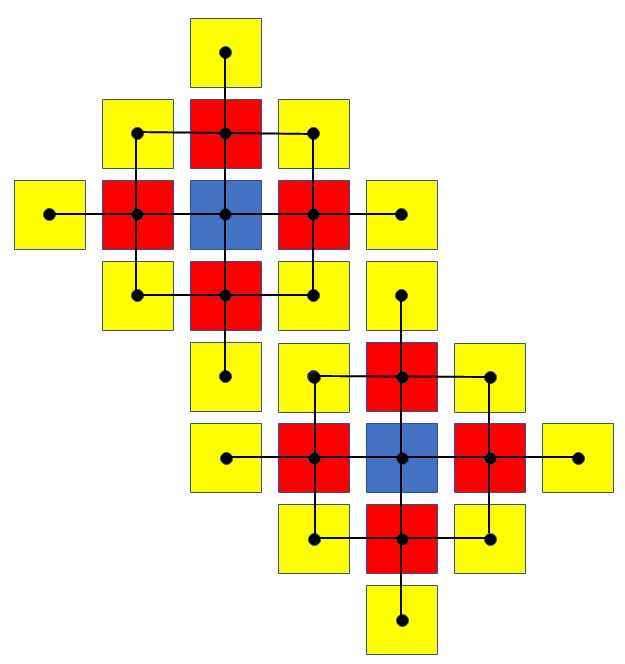
\includegraphics[width=0.99\linewidth]{Chapters/ProjROMs/Images/load_balancing_withEdgeCuts_noSyms.png}
    \end{minipage}
    \centering
    \begin{minipage}{0.45\linewidth}
        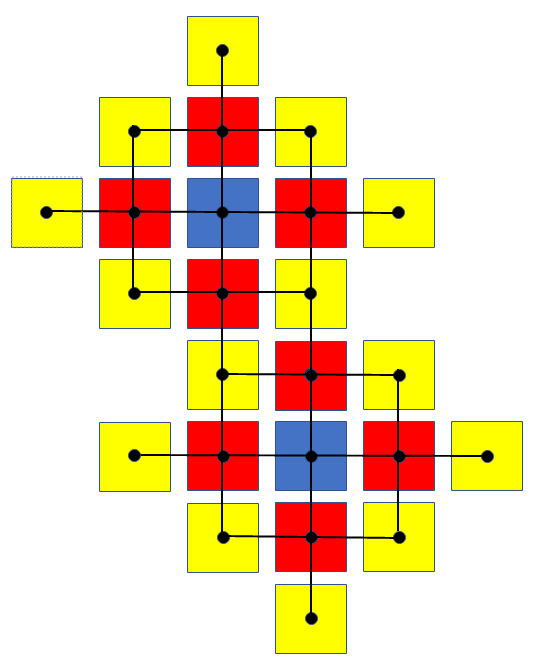
\includegraphics[width=0.99\linewidth]{Chapters/ProjROMs/Images/load_balancing_noEdgeCuts_noSyms.png}
    \end{minipage}
    \caption{\label{fig:edgeCuts}Mesh (graph) partitioning for load balancing. Some graph edges at finite volume cell faces can be excluded (left), while others are required (right).}
\end{figure}

As will be shown in Chapter~\ref{chap:CavityAndCVRC}, this approach to sample mesh partitioning can even lead to meshes which require zero MPI communications (besides collective operations). This occurs when sampling produces a number of small, disjoint graphs, i.e., individual graphs distributed in space which are not connected by any edges. On the other hand, fewer large, contiguous graphs arising from clustered sampling tend to result in fewer total nodes and smaller partition sizes, though they generally require more edge cuts to effectively load balance. The sparse sampling strategy can have a significant effect on this balance, as will be discussed in Chapter~\ref{chap:CavityAndCVRC}.
